\documentclass{beamer}
\usepackage{listings}
\lstset{
%language=C,
frame=single, 
breaklines=true,
columns=fullflexible
}
\usepackage{blkarray}
\usepackage{subcaption}
\usepackage{url}
\usepackage{tikz}
\usepackage{tkz-euclide} % loads  TikZ and tkz-base
%\usetkzobj{all}
\usetikzlibrary{calc,math}
\usepackage{float}
\newcommand\norm[1]{\left\lVert#1\right\rVert}
\renewcommand{\vec}[1]{\mathbf{#1}}
\usepackage[export]{adjustbox}
\usepackage[utf8]{inputenc}
\usepackage{amsmath}
\usepackage{tikz}
\usetikzlibrary{automata, positioning}
\usetheme{Boadilla}
\providecommand{\pr}[1]{\ensuremath{\Pr\left(#1\right)}}

\title{CSIR-UGC NET-Dec 2016-Problem(104)}
\author{Yashas Tadikamalla}
\date{AI20BTECH11027}
\begin{document}

\begin{frame}
\titlepage
\end{frame}

\begin{frame}
\frametitle{}
\begin{block}{Discrete-time Markov chains}
Consider a sequence of random variables $\{X_{t}\},t=0,1,2,\dots$, where $R_{X_{i}}=S\subset\{0,1,2,\dots\}$, $t$ denotes time. This sequence is said to be a Discrete-time Markov chain if it has the following property,
\begin{multline}
    \pr{X_{t+1}=j|X_{t}=i,X_{t-1}=i_{t-1},\dots,X_{0}=i_{0}}\\=\pr{X_{t+1}=j|X_{t}=i}
\end{multline}
$\forall j,i,i_{t-1},\dots,i_{0}$. If $S$ is finite, it is said to be a finite Discrete-time Markov chain.

\centering
\includegraphics[scale=0.20]{snake.jpg}
\end{block}
\end{frame}

\begin{frame}
\frametitle{}
\begin{block}{State transition matrix}
The state transition matrix is defined as
\begin{align}
\label{eq:pgen}
    P=\begin{blockarray}{cccccc}
&1 & 2 & 3 & \dots & r  \\
\begin{block}{c[ccccc]}
  1 & p_{11} & p_{12} & p_{13} & \dots & p_{1r} \\
  2 & p_{21} & p_{22} & p_{23} & \dots & p_{2r} \\
  3 & p_{31} & p_{32} & p_{33} & \dots & p_{3r} \\
  . & . & . & . & . & . \\
  . & . & . & . & . & . \\
  . & . & . & . & . & . \\
  r & p_{r1} & p_{r2} & p_{r3} & \dots & p_{rr} \\
\end{block}
\end{blockarray}
\end{align}
where, $p_{ij}=\pr{X_{t+1}=j|X_{t}=i},i,j\in S=\{1,2,\dots,r\}$.
\end{block}
\end{frame}

\begin{frame}
\frametitle{}
\begin{block}{n-step State transition matrix}
The n-step state transition matrix is defined as
\begin{align}
\label{eq:pngen}
    P^{(n)}=\begin{blockarray}{cccccc}
&1 & 2 & 3 & \dots & r  \\
\begin{block}{c[ccccc]}
  1 & p_{11}^{(n)} & p_{12}^{(n)} & p_{13}^{(n)} & \dots & p_{1r}^{(n)} \\
  2 & p_{21}^{(n)} & p_{22}^{(n)} & p_{23}^{(n)} & \dots & p_{2r}^{(n)} \\
  3 & p_{31}^{(n)} & p_{32}^{(n)} & p_{33}^{(n)} & \dots & p_{3r}^{(n)} \\
  . & . & . & . & . & . \\
  . & . & . & . & . & . \\
  . & . & . & . & . & . \\
  r & p_{r1}^{(n)} & p_{r2}^{(n)} & p_{r3}^{(n)} & \dots & p_{rr}^{(n)} \\
\end{block}
\end{blockarray}
\end{align}
where, $p_{ij}^{(n)}=\pr{X_{t+n}=j|X_{t}=i},i,j\in S=\{1,2,\dots,r\}$. 
\end{block}
\end{frame}

\begin{frame}
\frametitle{}
\begin{block}{Absorbing state}
A state is said to be absorbing, if the Markov chain, after attaining that state, remains in it forever. i.e, 
\begin{align}
    p_{ii}=1\Leftrightarrow\text{State i is absorbing}
\end{align}
\end{block}
\begin{block}{Non-absorbing state}
A state which is not absorbing, is said to be a non-absorbing state. i.e,
\begin{align}
    p_{ii}\neq 1\Leftrightarrow\text{State i is non-absorbing}
\end{align}
\end{block}
\begin{block}{Standard form of state transition matrix}
The standard form of a state transition matrix is
\begin{align}
\label{eq:std}
    P=\begin{blockarray}{ccc}
&A & N \\
\begin{block}{c[cc]}
  A & I & O  \\
  N & R & Q \\
\end{block}
\end{blockarray}
\end{align}
\end{block}
\end{frame}

\begin{frame}
\frametitle{}
\begin{block}{}
    \begin{table}[h!]
\centering
\caption{Notations and their meanings}
\label{table:2}
\begin{tabular}{|c|c|}
    \hline
    Notation & Meaning \\
    \hline
    $A$ & All absorbing states\\[1ex]
    \hline
    $N$ & All non-absorbing states\\[1ex]
    \hline
    $I$ & Identity matrix\\[1ex]
    \hline
    $O$ & Zero matrix\\[1ex]
    \hline
    $R,Q$ & Other submatices\\[1ex]
    \hline
\end{tabular}
\end{table}
\end{block}
%\begin{block}{}
%The following rule applies to all types of state transition matrices
%\begin{align}
%\label{eq:sum}
%    \displaystyle\sum_{j=0}^{r}p_{ij}=1,\forall i\in S
%\end{align}
%\end{block}
\end{frame}

\begin{frame}
\frametitle{Question}
\begin{block}{CSIR-UGC NET-Dec 2016-Problem(104)}
$A$ and $B$ play a game of tossing a fair coin. $A$ starts the game by tossing the coin once and $B$ then tosses the coin twice, followed by $A$ tossing the coin once and $B$ tossing the coin twice and this continues until a head turns up. Whoever gets the first head wins the game. Then, 
\begin{enumerate}
    \item $P(B$ Wins) $> P(A$ Wins)
    \item $P(B$ Wins) $= 2P(A$ Wins)
    \item $P(A$ Wins) $> P(B$ Wins)
    \item $P(A$ Wins) $= 1-P(B$ Wins)
\end{enumerate}
\end{block}
\end{frame}

\begin{frame}
\frametitle{Solution}
Given, a fair coin is tossed till heads turns up.
\begin{align}
\label{eq:0}
    \pr{H}=p=\dfrac{1}{2}\\\pr{T}=q=\dfrac{1}{2}
\end{align}
According to the question, until a player wins, the following set of events occur repetitively, 
\begin{enumerate}
    \item Player $A$'s turn
    \item Player $B$'s first turn
    \item Player $B$'s second turn
\end{enumerate}
\end{frame}

\begin{frame}
\frametitle{Solution Contd.}
Let's define the problem as a finite Markov chain $\{X_{t}\},t=0,1,2,\dots$, where $R_{X_{i}}=S=\{1,2,3,4,5\}$
such that
\begin{table}[h!]
\centering
\caption{States and their notations}
\label{table:1}
\begin{tabular}{|c|c|}
    \hline
    Notation & State \\
    \hline
    $S=1$ & $A$'s turn\\[1ex]
    \hline
    $S=2$ & $B$'s first turn\\[1ex]
    \hline
    $S=3$ & $B$'s second turn\\[1ex]
    \hline
    $S=4$ & $A$ wins\\[1ex]
    \hline
    $S=5$ & $B$ wins\\[1ex]
    \hline
\end{tabular}
\end{table}
\end{frame}

\begin{frame}
\frametitle{Solution Contd.}
The state transition matrix for the above Markov chain is
\begin{align}
\label{eq:p}
    P=\begin{blockarray}{cccccc}
&1 & 2 & 3 & 4 & 5 \\
\begin{block}{c[ccccc]}
  1 & 0 & 0.5 & 0 & 0.5 & 0 \\
  2 & 0 & 0 & 0.5 & 0 & 0.5 \\
  3 & 0.5 & 0 & 0 & 0 & 0.5 \\
  4 & 0 & 0 & 0 & 1 & 0 \\
  5 & 0 & 0 & 0 & 0 & 1 \\
\end{block}
\end{blockarray}
\end{align}
Clearly, the states $4,5$ are absorbing, while $1,2,3$ are non-absorbing.
\end{frame}

\begin{frame}
\frametitle{Solution Contd.}
Converting \eqref{eq:p} into standard form gives
\begin{align}
\label{eq:pstd}
    P=\begin{blockarray}{cccccc}
&4 & 5 & 1 & 2 & 3 \\
\begin{block}{c[ccccc]}
  4 & 1 & 0 & 0 & 0 & 0 \\
  5 & 0 & 1 & 0 & 0 & 0 \\
  1 & 0.5 & 0 & 0 & 0.5 & 0 \\
  2 & 0 & 0.5 & 0 & 0 & 0.5 \\
  3 & 0 & 0.5 & 0.5 & 0 & 0 \\
\end{block}
\end{blockarray}
\end{align}
Comparing \eqref{eq:pstd} with \eqref{eq:std}, we get
\begin{align}
\label{eq:r,q}
    R=\begin{bmatrix}
    0.5 & 0\\
    0 & 0.5\\
    0 & 0.5\\
    \end{bmatrix},
    Q=\begin{bmatrix}
    0 & 0.5 & 0\\
    0 & 0 & 0.5\\
    0.5 & 0 & 0\\
    \end{bmatrix}
\end{align}
\end{frame}

\begin{frame}
\frametitle{}
    \begin{block}{Limiting matrices for absorbing Markov chains}
    If $P$ is the state transition matrix in standard form, i.e,
    \begin{align}
         P=\begin{bmatrix}
    I & O\\
    R & Q\\
    \end{bmatrix}
    \end{align}
    then $P^{(K)}$ approaches $\bar P$ as k increases. 
    \begin{align}
        \displaystyle\lim_{k\to\infty}P^{(K)}=\bar P
    \end{align}
    where,
    \begin{align}
        \label{eq:pbar}
    \bar P=\begin{bmatrix}
    I & O\\
    FR & O\\
    \end{bmatrix},
    F=(I-Q)^{-1}
    \end{align}
    $F$ is called the fundamental matrix of $P$.  
    \end{block}
\end{frame}

 \begin{frame}
 \frametitle{Solution Contd.}
 Solving \eqref{eq:r,q},\eqref{eq:pbar}, we get
 \begin{align}
\label{eq:ans}
    \bar P=\begin{blockarray}{cccccc}
&4 & 5 & 1 & 2 & 3 \\
\begin{block}{c[ccccc]}
    4 & 1 & 0 & 0 & 0 & 0 \\
    5 & 0 & 1 & 0 & 0 & 0 \\[1ex]
    1 & \frac{4}{7} & \frac{3}{7} & 0 & 0 & 0 \\[1ex]
    2 & \frac{1}{7} & \frac{6}{7} & 0 & 0 & 0 \\[1ex]
    3 & \frac{2}{7} & \frac{5}{7} & 0 & 0 & 0 \\[1ex]
   \end{block}
\end{blockarray}
\end{align}
 A element $\bar p_{ij}$ of $\bar P$ denotes the absorption probability in state $j$, starting from state $i$. 
\end{frame}

\begin{frame}
 \frametitle{Solution Contd.}
 Therefore
 \begin{enumerate}
    \item $\pr{\text{\textit{A} wins}}=\bar p_{14}=\dfrac{4}{7}$
    \item $\pr{\text{\textit{B} wins}}=\bar p_{15}=\dfrac{3}{7}$
\end{enumerate}
 Clearly,
\begin{align}
\bar p_{14} > \bar p_{15}
\end{align}
and
\begin{align}
\bar p_{14}=1-\bar p_{15}
\end{align}
Therefore, options $3,4$ are correct.
\end{frame}

\begin{frame}
 \frametitle{Solution Contd.}
 Theoretical vs Simulation plot
\centering
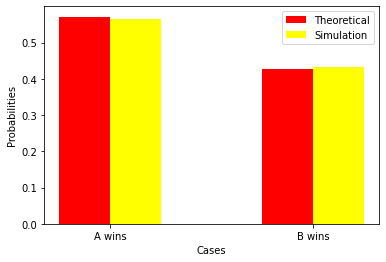
\includegraphics[scale=0.65]{Assignment8.png}
 \end{frame}
 
 \begin{frame}
 \frametitle{Solution Contd.}
 \begin{figure}[h]
\caption*{\textbf{Markov chain diagram}}
\centering
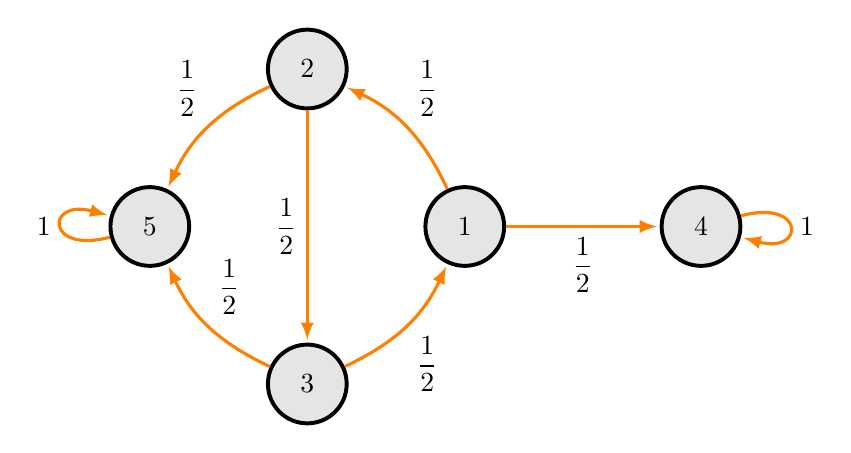
\begin{tikzpicture}
    % Setup the style for the states
        \tikzset{node style/.style={state, 
                                    minimum width=1cm,
                                    line width=0.5mm,
                                    fill=gray!20!white}}
        % Draw the states
        \node[node style] at (4,-2)      (bull)     {1};
        \node[node style] at (2,0)      (bear)     {2};
        \node[node style] at (2, -4) (stagnant) {3};
        \node[node style] at (7,-2) (over1) {4};
        \node[node style] at (0, -2) (over2) {5};
        % Connect the states with arrows
        \draw[every loop,
              auto=right,
              line width=0.4mm,
              >=latex,
              draw=orange,
              fill=orange]
            (stagnant)     edge[bend right=20]            node {$\dfrac{1}{2}$} (bull)
            (stagnant)     edge[bend left=20]            node {$\dfrac{1}{2}$} (over2)
            (bull)     edge[bend right=20] node {$\dfrac{1}{2}$} (bear)
            (bull)     edge node {$\dfrac{1}{2}$} (over1)
            (bear)     edge[bend right=20] node {$\dfrac{1}{2}$} (over2)
            (bear)     edge node {$\dfrac{1}{2}$} (stagnant)
            (over1) edge[loop right]             node  {1} (over1)
            (over2) edge[loop left]             node  {1} (over2);
\end{tikzpicture}
\end{figure}
 \end{frame}

\end{document}